\documentclass{unicam_thesis}
\usepackage[utf8]{inputenc}
\usepackage{listings}
\usepackage{braket}
\usepackage[backend=bibtex]{biblatex}
\usepackage[automake,toc,acronyms,nonumberlist, nopostdot]{glossaries}
\usepackage{mathabx}
\usepackage{amsthm}
\usepackage{graphicx} 
\usepackage{tikz}  
\usetikzlibrary{quantikz, positioning, arrows.meta, calc, automata, positioning, backgrounds, fit, shapes.geometric}
\usepackage{booktabs}     
\usepackage{subcaption}  
\usepackage{amsthm}
\usepackage{adjustbox}
\usepackage{amssymb}
\usepackage[utf8]{inputenc}
\usepackage[T1]{fontenc}
\usepackage{lmodern}
\usepackage[nottoc]{tocbibind}
\usepackage{hyperref}


\theoremstyle{plain}
\newtheorem{theorem}{Theorem}[section]
\newtheorem{lemma}{Lemma}[section]
\newtheorem{corollary}{Corollary}[section]
\newtheorem{proposition}{Proposition}[section]
\newtheorem{conjecture}{Conjecture}[section]
\newtheorem{assumption}{Assumption}[section]

\theoremstyle{definition}
\newtheorem{definition}{Definition}[section]
\newtheorem{example}{Example}[section]
\newtheorem{exercise}{Exercise}[section]
\newtheorem{algorithm}{Algorithm}[section]
\newtheorem{concept}{Concept}[section]

\theoremstyle{remark}
\newtheorem*{remark}{Remark}
\newtheorem{observation}{Observation}[section]
\newtheorem{notation}{Notation}[section]



\tikzset{rejecting/.style={circle, draw, red, dashed}}

\makeglossaries
\loadglsentries[acronym]{myglossaries}

\title{Systematic Taxonomy of Quantum Finite Automata: Bridging Classical and Quantum Computational Models}

\university{Universit\`a degli Studi di Camerino}
\school{Scienze e Tecnologie}
\course{Laurea in Informatica (Classe L-31)}


\author{Marta Musso}
\advisor{Relatore Name}
% add Marcello Bonsangue, Michele Loreti
\coadvisor2{Correlatore Name}
\academicyear{2024/2025}
\matricola{122360}

\graphicspath{{Screenshot/},{Pictures/},{API/},{Source/}}
\addbibresource{biblio.bib}
\begin{document}

\maketitle
\begin{abstract} {
    Quantum automata theory investigates how principles of quantum mechanics can be integrated with classical models of computation to reveal new limits and possibilities in computational power. Although the theory offers deep insights, progress has been slowed by inconsistent notation, unclear model definitions, and fragmented comparisons across different approaches. This thesis establishes a unified framework that standardises definitions and systematically compares classical finite automata with their quantum counterparts, focusing on state complexity and language recognition capabilities.

    The work begins with a comprehensive review of classical finite automata, including deterministic, nondeterministic, probabilistic, and two-way models, also specifying the formal language theory that underpins these models. This review lays the necessary theoretical foundation for the subsequent discussion of quantum finite automata.
    The thesis then introduces the foundational principles of quantum mechanics and explains how these underpin the definition of quantum automata. 
    Subsequently, the work reviews various quantum automata models, analyzing their formal definitions, computational dynamics and language recognition properties. 
    Lastly, the thesis presents a unified taxonomy that provides a systematic comparison between classical and quantum automata models, highlighting the computational capabilities and limitations of quantum automata.
    The unified framework presented here offers clear insights into the computational capabilities and limitations of quantum automata, and it provides a systematic basis for further research in quantum computational models.
}

\noindent\textbf{Keywords:} Quantum automata, finite automata taxonomy, computational complexity, hybrid quantum-classical models, formal language theory 
\end{abstract}
\newpage


\tableofcontents

%\lstlistoflistings
%\listoffigures
%\listoftables

\chapter{Introduction}  
\label{chap:introduction}

The intersection of quantum mechanics and theoretical computer science has given rise to quantum computing, a field that reimagines computational paradigms through the lens of quantum phenomena such as superposition and entanglement. At its core lies quantum automata theory, which seeks to understand how these principles redefine the boundaries of classical computation. \glspl{cfa}—\gls{dfa}, \gls{nfa}, \gls{pfa}, and two-way variants—have long served as the bedrock of formal language theory, offering mathematically rigorous frameworks for analyzing computational complexity and decidability. In contrast, \glspl{qfa} exhibit probabilistic and non-deterministic behaviors that transcend classical limits, necessitating a coherent framework to classify and analyse their capabilities. This thesis emerges from the recognition that the current landscape of quantum automata theory is fragmented: definitions vary across papers, notations lack standardization, and comparisons between classical and quantum models remain scattered across disjointed works \cite{gruska2012quantum}. By systematically unifying these elements, this thesis aims to bridge the conceptual gap between classical and quantum computational models, offering a structured lens through which their interaction can be rigorously studied \cite{ambainis2009superiority}.  

The motivation for this work is two-fold: theoretical exploration and practical application. Theoretically, quantum automata represent the simplest quantum computational models, providing a sandbox to explore the interplay between quantum mechanics and computation. They challenge classical intuitions—for instance, quantum parallelism enables certain \glspl{qfa}, such as the \gls{mm-1qfa}, to recognise languages with exponentially fewer states than their classical counterparts \cite{ambainis1998one}. Practically, as quantum hardware advances, understanding the minimal resources required to implement \glspl{qfa} becomes critical for designing efficient algorithms and robust error-correcting schemes \cite{nielsen2010quantum}. Yet, progress in the field has been hindered by ambiguities in model definitions. For example, early quantum automata models like the \gls{mo-1qfa} and \gls{mm-1qfa} were defined with differing acceptance criteria, leading to confusion about their relative computational power \cite{kondacs1997power}. Similarly, hybrid models such as the \gls{1qfac} introduce classical memory components, complicating direct comparisons to purely quantum or classical automata \cite{li2012characterizations}. These inconsistencies obscure the true capabilities of quantum models and hinder cross-disciplinary collaboration.

A central observation motivating this thesis is that no single document currently catalogs quantum automata models alongside their classical counterparts. Existing surveys, while valuable, often focus on specific subsets of models or lack the granularity needed to resolve nuanced differences in computational power, closure properties, or decidability \cite{gruska2012quantum}. For instance, although the expressive power of \gls{2qfa} surpasses that of classical two-way automata, the conditions under which this advantage manifests—such as the role of quantum interference in recognizing non-regular languages—remain underexplored in a unified context \cite{yakaryilmaz2010succinctness}. Moreover, the literature review in this thesis is dedicated to clearly identifying the specific classes of languages each automaton model accepts. In contrast, this work adopts a taxonomic approach, dissecting each model’s formal definition, acceptance criteria, and operational dynamics while contextualizing its position within the broader hierarchy of automata. This approach not only clarifies existing results but also identifies gaps where further research is needed, such as the decidability of equivalence problems for \glspl{qfa} with mixed states or the precise trade-offs between quantum entanglement and space efficiency \cite{hirvensalo2012quantum}.  

The research challenges addressed in this thesis are multifaceted. First, reconciling disparate notation and definitions requires a meticulous synthesis of foundational and contemporary literature. For example, the transition from unitary operations in \gls{mo-1qfa} to superoperator-based transitions in open quantum systems, as seen in \glspl{otqfa}, calls for a unified formalism to compare their computational behaviors \cite{bertoni2001quantum, breuer2002theory}. Second, characterizing the relationships between classical and quantum models necessitates a framework that accounts for both their similarities (e.g., the ability of \gls{1qfac} to simulate \glspl{dfa}) and their divergences (e.g., the exponential state advantage of \gls{2qfa} over two-way probabilistic automata). Third, the absence of standardised pumping lemmas or minimization algorithms for \glspl{qfa} complicates efforts to classify their language recognition capabilities, a challenge that this thesis tackles through a comparative analysis of closure properties and equivalence criteria \cite{yakaryilmaz2014quantum}.  

To address these challenges, this thesis employs a structured methodology that unfolds in several stages. It begins by grounding the discussion in classical automata theory, revisiting \gls{dfa}, \gls{nfa}, \gls{pfa}, and two-way variants to establish foundational concepts. Building on this, the thesis introduces the foundational principles of quantum mechanics—such as superposition, entanglement, and measurement—which provide the basis for defining quantum finite automata \cite{nielsen2010quantum}. With this dual background in place, the work systematically explores various quantum models, ranging from early variants like the \gls{mo-1qfa} \cite{moore2000quantum} and the \gls{mm-1qfa} \cite{kondacs1997power} to advanced hybrids such as the \gls{1qfac} and enhanced models (e.g., the \gls{eqfa}). Each model is rigorously analysed along several dimensions: its formal definition is standardised, its acceptance criteria are scrutinised, and its computational dynamics—such as the role of measurement timing and the interplay between quantum and classical states—are carefully dissected, with particular emphasis on identifying the exact classes of formal languages recognised by each model.

A significant contribution of this work is the development of a hierarchical taxonomy of automata models, which organises both classical and quantum automata into a coherent structure based on their computational features and complexity classes. For example, the analysis reveals that \glspl{2qfa} occupy a higher complexity class than their one-way counterparts, while hybrid models such as the \gls{1qfac} serve as an intermediate bridge between purely quantum and purely classical models \cite{yakaryilmaz2010succinctness}. The taxonomy further highlights open research questions, such as the precise relationships between models that employ different quantum operational frameworks (e.g., \glspl{a-qfa} versus \glspl{gqfa}) and the conditions under which quantum automata outperform probabilistic models in language recognition tasks \cite{hirvensalo2012quantum}.

The thesis is organised to guide the reader through these progressively complex layers of analysis. Following this introduction, Chapter~\ref{chap:background} consolidates foundational concepts from both classical automata theory and quantum mechanics, providing a unified background for the discussions that follow. Chapter~\ref{chap:literature-review} presents a comprehensive catalog of quantum automata models; each model is formally defined, its computational dynamics are analysed, and its language recognition capabilities are explicitly detailed. Chapter~\ref{chap:comparative-analysis} synthesises these findings by evaluating expressive power, closure properties, and decidability issues across different models. Finally, Chapter~\ref{chap:conclusion} concludes by reflecting on the thesis’s contributions and outlining directions for future research, such as solving open questions in equivalence checking for \glspl{qfa} \cite{li2012characterizations}, extending pumping lemmas to quantum models \cite{yakaryilmaz2014quantum}, and developing minimization algorithms for hybrid automata.

In essence, this thesis seeks to transform quantum automata theory from a collection of isolated results into a cohesive and systematic framework. By standardizing definitions, clarifying the relationships between different models, and identifying critical open challenges, the work provides both a valuable reference for researchers and a solid methodological basis for future advancements in quantum computational models. As quantum computing transitions from theory to practice, such systematic foundations will be essential for harnessing the full potential of quantum-enhanced computation.
\chapter{Background}  

The study of quantum automata theory necessitates a thorough grounding in both classical computational models and the quantum mechanical principles that redefine their capabilities. This chapter systematically establishes the conceptual foundation for analyzing quantum automata by first revisiting classical finite automata—the cornerstone of formal language theory—and then introducing the quantum mechanical framework that enables novel computational paradigms.

We begin with an in-depth exploration of classical finite automata, which serve as the theoretical bedrock for understanding computational limits and language recognition. Deterministic finite automata (DFAs), non-deterministic finite automata (NFAs), probabilistic finite automata (PFAs), and their two-way variants are analyzed through their formal definitions, operational dynamics, and closure properties. These models collectively define the boundaries of classical computation, particularly in recognizing regular languages and their limitations in handling context-free or stochastic languages. The analysis draws on foundational works such as Hopcroft et al. \cite{hopcroft2006introduction}, which formalized the equivalence between DFAs and NFAs, and Rabin's seminal work on probabilistic automata \cite{rabin1963probabilistic}, which expanded the class of recognizable languages through probabilistic acceptance criteria.

The discourse then transitions to quantum mechanical principles essential for quantum computation. Key concepts such as qubit representation, quantum superposition, and entanglement are contextualized within computational frameworks, emphasizing their departure from classical bit-based processing. The measurement postulate and its implications for probabilistic outcomes are discussed in relation to quantum state collapse, a critical distinction from classical probabilistic models. These principles are synthesized with insights from Nielsen and Chuang's definitive text on quantum computation \cite{nielsen2010quantum}, which provides the mathematical formalism for quantum operations.

The chapter's structure is designed to mirror the hierarchical taxonomy developed in later chapters. By first rigorously defining classical models and their limitations, followed by an exposition of quantum principles and their computational implications, the groundwork is laid for analyzing hybrid models such as the one-way quantum finite automaton with classical states (1QFAC) \cite{zheng2012one}. Each section deliberately connects theoretical constructs to practical considerations, such as the role of decoherence in open quantum systems \cite{breuer2002theory} and its impact on automata design. This approach ensures that subsequent discussions of quantum automata variants are rooted in both mathematical rigor and physical realizability.

\section{Classical Finite Automata}
\label{sec:classical-finite-automata} 

Finite automata form the cornerstone of formal language theory, providing mathematical frameworks to analyze computational limits and language recognition capabilities. This section systematically examines deterministic, nondeterministic, probabilistic, and two-way variants, emphasizing their structural relationships and computational boundaries. 

\subsection{Shared Foundations}
\label{subsec:shared-foundations} 

The study of automata begins with foundational concepts in formal language theory. An \textit{alphabet} $\Sigma$ is a finite set of symbols (e.g., $\Sigma = \{0,1\}$), while a \textit{string} $w$ over $\Sigma$ is a finite sequence of symbols with length $\|w\|$ \cite{hopcroft2006introduction}. The empty string $\epsilon$ has $\|\epsilon\| = 0$. A \textit{language} $L$ is a set of strings, i.e., $L \subseteq \Sigma^\ast$, where $\Sigma^\ast$ denotes the Kleene closure—the set of all finite strings over $\Sigma$ \cite{hopcroft2006introduction}. Key operations include:
\begin{itemize}
    \item \textit{Concatenation}: Combining strings $u$ and $v$ into $uv$.
    \item \textit{Union/Intersection}: $L_1 \cup L_2$ and $L_1 \cap L_2$.
    \item \textit{Kleene Star}: $L^\ast = \bigcup_{i=0}^\infty L^i$, where $L^0 = \{\epsilon\}$ \cite{hopcroft2006introduction}.
\end{itemize} 

Languages are categorized by recognition models:
\begin{itemize}
    \item \textit{Regular languages ($\text{REG}$)}: Recognized by DFAs, NFAs, or regular expressions \cite{hopcroft2006introduction}.
    \item \textit{Stochastic languages}: Recognized by probabilistic finite automata (PFAs) with bounded error \cite{rabin1963probabilistic}.
\end{itemize} 

Regular languages exhibit critical closure properties under union, intersection, complement, concatenation, and Kleene star \cite{hopcroft2006introduction}. These properties underpin decidability proofs and equivalence checks, forming the basis for analyzing quantum automata in later chapters. 

\subsection{Deterministic Finite Automata (DFA)}
\label{subsec:dfa} 

A DFA is a quintuple $M = (Q, \Sigma, \delta, q_0, F)$, where:
\begin{itemize}
    \item $Q$: Finite set of states.
    \item $\Sigma$: Input alphabet.
    \item $\delta: Q \times \Sigma \to Q$: Deterministic transition function.
    \item $q_0 \in Q$: Initial state.
    \item $F \subseteq Q$: Accepting states \cite{hopcroft2006introduction}.
\end{itemize} 

Computation proceeds deterministically: for input $w = a_1 a_2 \dots a_n$, the state evolves as $\delta(q_{i-1}, a_i) = q_i$ \cite{hopcroft2006introduction}. A string $w$ is accepted if $\delta(q_0, w) \in F$. DFAs recognize precisely the regular languages, with expressive power strictly weaker than context-free languages \cite{hopcroft2006introduction}. 

Key properties include:
\begin{itemize}
    \item \textit{Minimization}: Hopcroft's algorithm reduces DFAs to minimal form in $O(n \log n)$ time \cite{hopcroft2006introduction}.
    \item \textit{Emptiness Problem}: Decidable via reachability analysis from $q_0$ to $F$ \cite{hopcroft2006introduction}.
    \item \textit{Pumping Lemma}: For any $L \in \text{REG}$, there exists $p$ such that any $w \in L$ with $\|w\| \geq p$ can be decomposed as $w = xyz$ (with $\|xy\| \leq p$, $\|y\| \geq 1$) such that $xy^i z \in L$ for all $i \geq 0$ \cite{hopcroft2006introduction}.
\end{itemize} 

\subsection{Nondeterministic Finite Automata (NFA)}
\label{subsec:nfa} 

NFAs generalize DFAs by allowing multiple transitions per input symbol. Formally, an NFA is a quintuple $M = (Q, \Sigma, \delta, q_0, F)$, where $\delta: Q \times (\Sigma \cup \{\epsilon\}) \to 2^Q$ enables $\epsilon$-transitions and nondeterministic branching \cite{hopcroft2006introduction}. A string $w$ is accepted if \textit{any} computational path leads to $F$. 

Despite apparent increased power, NFAs recognize the same class of languages as DFAs ($\text{REG}$) \cite{hopcroft2006introduction}. However, they can be exponentially more succinct: for example, an NFA recognizing $\{w \mid w \text{ contains } ab\}$ requires only $3$ states, while the equivalent DFA requires $2^3 = 8$ states \cite{hopcroft2006introduction}. Subset construction converts an NFA with $n$ states to a DFA with up to $2^n$ states \cite{hopcroft2006introduction}. 

NFAs inherit closure properties from DFAs but lack unique minimization—equivalence checks require conversion to DFAs \cite{hopcroft2006introduction}. 

\subsection{Probabilistic Finite Automata (PFA)}
\label{subsec:pfa} 

PFAs introduce probabilistic transitions. A PFA is defined as $M = (Q, \Sigma, \delta, q_0, F)$, where $\delta: Q \times \Sigma \times Q \to [0, 1]$ specifies transition probabilities \cite{rabin1963probabilistic}. A string $w$ is accepted if the probability of ending in $F$ exceeds a threshold $\lambda \in [0, 1]$ \cite{rabin1963probabilistic}. 

PFAs recognize \textit{stochastic languages} (a superset of $\text{REG}$), including non-regular languages like $L_{eq} = \{a^n b^n \mid n \geq 1\}$ with bounded error \cite{rabin1963probabilistic}. However, their computational power comes at a cost:
\begin{itemize}
    \item \textit{Emptiness Problem}: Undecidable—no algorithm can determine if $\Pr[\text{accept}] > 0$ \cite{paz1971introduction}.
    \item \textit{Equivalence}: Undecidable for PFAs, unlike DFAs/NFAs \cite{paz1971introduction}.
\end{itemize} 

These limitations highlight the trade-offs between expressiveness and decidability in probabilistic models. 

\subsection{Two-Way Finite Automata (2DFA, 2NFA, 2PFA)}
\label{subsec:2dfa} 

Two-way automata extend finite automata with bidirectional tape heads. A 2DFA is defined as $M = (Q, \Sigma, \delta, q_0, F)$, where $\delta: Q \times \Sigma \to Q \times \{L, R\}$ governs state transitions and head movement \cite{kondacs1997power}. Despite this added capability, 2DFAs recognize only $\text{REG}$, though they can achieve exponential state savings for certain languages \cite{kondacs1997power}. 

Two-way probabilistic finite automata (2PFAs) significantly enhance power. For example, a 2PFA recognizes $L_{eq} = \{a^n b^n\}$ with bounded error in polynomial time, a feat impossible for one-way PFAs \cite{kondacs1997power}. However, 2PFAs sacrifice decidability:
\begin{itemize}
    \item \textit{Emptiness Problem}: Undecidable due to probabilistic ambiguity \cite{kondacs1997power}.
    \item \textit{Equivalence}: Undecidable for 2PFAs \cite{kondacs1997power}.
\end{itemize} 

These models bridge classical and quantum automata, as their bidirectional access prefigures quantum interference effects in 2QFAs \cite{ambainis2009superiority}. 

\subsection{Key Theorems}
\label{subsec:key-theorems} 

\begin{enumerate}
    \item \textit{Kleene's Theorem}: A language is regular if and only if it is recognized by a DFA/NFA or described by a regular expression \cite{hopcroft2006introduction}.
    \item \textit{Subset Construction Theorem}: Every NFA can be converted to an equivalent DFA, with up to $2^n$ states \cite{hopcroft2006introduction}.
    \item \textit{Myhill-Nerode Theorem}: Characterizes $\text{REG}$ via string indistinguishability, forming the basis for DFA minimization \cite{hopcroft2006introduction}.
    \item \textit{Rabin's Theorem}: PFAs recognize stochastic languages, a strict superset of $\text{REG}$ \cite{rabin1963probabilistic}.
    \item \textit{Sipser's Theorem}: 2PFAs recognize $\text{REG}$ in logarithmic space but require exponential time for non-regular languages \cite{sipser1980halting}.
\end{enumerate} 

These theorems collectively delineate the boundaries of classical finite automata, setting the stage for quantum extensions in subsequent chapters. 
\section{Quantum Mechanics Foundations}
\label{sec:quantum-foundations}

This section establishes the quantum mechanical principles underpinning quantum automata theory, emphasizing mathematical formalism and conceptual distinctions from classical systems. The discussion focuses on foundational postulates and their computational implications.

\subsection{Qubits and Quantum States}
\label{subsec:qubits}

A \textit{qubit} is the quantum analog of a classical bit, represented by a unit vector in a two-dimensional complex Hilbert space $\mathcal{H} = \mathbb{C}^2$ \cite{nielsen2010quantum}. The standard basis states are denoted:
\[
|0\rangle = \begin{pmatrix} 1 \\ 0 \end{pmatrix}, \quad |1\rangle = \begin{pmatrix} 0 \\ 1 \end{pmatrix},
\]
with general qubit states expressed as:
\[
|\psi\rangle = \alpha|0\rangle + \beta|1\rangle, \quad |\alpha|^2 + |\beta|^2 = 1,
\]
where $\alpha, \beta \in \mathbb{C}$ are the probability amplitudes \cite{nielsen2010quantum}. Geometrically, the qubit states correspond to points on the \textit{Bloch sphere}:
\[
|\psi\rangle = \cos\frac{\theta}{2}|0\rangle + e^{i\phi}\sin\frac{\theta}{2}|1\rangle,
\]
parameterized by polar angles $\theta \in [0, \pi]$ and $\phi \in [0, 2\pi)$ \cite{nielsen2010quantum}. Multi-qubit systems are described by tensor products, e.g., a two-qubit state:
\[
|\psi\rangle = \sum_{i,j \in \{0,1\}} \alpha_{ij}|i\rangle \otimes |j\rangle, \quad \sum_{i,j} |\alpha_{ij}|^2 = 1.
\]

\subsection{Superposition and Entanglement}
\label{subsec:superposition}

\textit{Superposition} allows qubits to exist in linear combinations of basis states, enabling parallel processing of multiple states \cite{nielsen2010quantum}. For example, the Hadamard gate $H$ creates superposition from classical states:
\[
H|0\rangle = \frac{|0\rangle + |1\rangle}{\sqrt{2}}, \quad H|1\rangle = \frac{|0\rangle - |1\rangle}{\sqrt{2}}.
\]
\textit{Entanglement} arises when qubits exhibit non-classical correlations. The Bell state:
\[
|\Phi^+\rangle = \frac{|00\rangle + |11\rangle}{\sqrt{2}},
\]
cannot be factored into tensor products of individual qubit states, violating Bell's inequality and enabling quantum teleportation protocols \cite{nielsen2010quantum}. Entanglement is a critical resource for quantum speedups in automata models like 2QFAs \cite{ambainis2009superiority}.

\subsection{Quantum Gates and Circuits}
\label{subsec:gates}

Quantum operations are performed via \textit{unitary transformations} $U$ satisfying $U^\dagger U = I$. Common single-qubit gates include:
\begin{itemize}
    \item Pauli-X: $X = \begin{pmatrix} 0 & 1 \\ 1 & 0 \end{pmatrix}$ (bit flip).
    \item Hadamard: $H = \frac{1}{\sqrt{2}}\begin{pmatrix} 1 & 1 \\ 1 & -1 \end{pmatrix}$.
    \item Phase shift: $R_\phi = \begin{pmatrix} 1 & 0 \\ 0 & e^{i\phi} \end{pmatrix}$.
\end{itemize}
Two-qubit gates, such as the controlled-NOT (CNOT):
\[
\text{CNOT}|a\rangle|b\rangle = |a\rangle|a \oplus b\rangle,
\]
enable entanglement generation \cite{nielsen2010quantum}. Quantum circuits compose these gates to implement algorithms, with depth and width determining computational complexity.

\subsection{Measurement and Probabilistic Outcomes}
\label{subsec:measurement}

Measurement collapses a quantum state to a classical outcome. For an orthonormal basis $\{|i\rangle\}$, measuring $|\psi\rangle = \sum_i \alpha_i|i\rangle$ yields outcome $i$ with probability $|\alpha_i|^2$ (Born rule) \cite{nielsen2010quantum}. For example, measuring $|\Phi^+\rangle$ in the computational basis gives $|00\rangle$ or $|11\rangle$ with equal probability. Unlike classical randomness, measurement outcomes depend on the chosen basis, a feature exploited in quantum automata's acceptance criteria \cite{moore2000quantum}.

\subsection{Decoherence and Open Systems}
\label{subsec:decoherence}

Real quantum systems interact with environments, causing \textit{decoherence}—the loss of coherence in superposition states \cite{breuer2002theory}. The Lindblad master equation models open system dynamics:
\[
\frac{d\rho}{dt} = -\frac{i}{\hbar}[H, \rho] + \sum_k \left( L_k \rho L_k^\dagger - \frac{1}{2}\{L_k^\dagger L_k, \rho\} \right),
\]
where $\rho$ is the density matrix and $L_k$ are Lindblad operators \cite{breuer2002theory}. Decoherence limits quantum automata's operational timeframes, necessitating error correction or hybrid classical-quantum designs \cite{zheng2012one}.
\chapter{Literature Review}
\label{chap:chapter3}

\section{One-way QFAs}
\label{sec:one-way-qfas}

\subsection{Standard Models}
\label{subsec:standard-models}

\subsubsection{MO-1QFA (Measure-Once)}
\label{sssec:mo-1qfa}

\textbf{Definition}: An MO-1QFA is defined as \( M = (Q, \Sigma, \delta, q_0, F) \), where:
- \( Q \): Finite set of quantum basis states.
- \( \Sigma \): Input alphabet with end-marker \( \# \).
- \( \delta \): Transition function inducing unitary operators \( U_\sigma \) for \( \sigma \in \Sigma \).
- \( q_0 \in Q \): Initial state.
- \( F \subseteq Q \): Accepting states \cite{moore2000quantum}.

\textbf{Operation}: Processes input sequentially with a single measurement at the end. The state evolves as \( |\psi_i\rangle = U_{\sigma_i}|\psi_{i-1}\rangle \). Acceptance is determined by projecting onto \( F \) \cite{moore2000quantum}.

\textbf{Key Features}:
- Recognizes a strict subset of regular languages (e.g., periodic languages) \cite{bertoni2001regular}.
- Requires \( O(n) \) states for languages like \( L_{\text{mod}} = \{w \mid |w| \equiv 0 \mod p\} \).

\textbf{Limitations}: 
- Cannot recognize non-regular languages like \( L_{\text{eq}} = \{a^n b^n\} \).

\subsubsection{MM-1QFA (Measure-Many)}
\label{sssec:mm-1qfa}

\textbf{Definition}: An MM-1QFA is \( M = (Q, \Sigma, \delta, q_0, Q_{\text{acc}}, Q_{\text{rej}}, Q_{\text{non}}) \), where:
- \( Q_{\text{acc}}, Q_{\text{rej}}, Q_{\text{non}} \): Partitioned states for halting and continuation \cite{kondacs1997power}.

\textbf{Operation}: Measures after each symbol, halting if \( Q_{\text{acc}} \) or \( Q_{\text{rej}} \) is observed \cite{kondacs1997power}.

\textbf{Key Features}:
- Recognizes non-regular languages (e.g., \( L_{\text{eq}} \)) with bounded error \cite{kondacs1997power}.
- Exponential state advantage over DFAs for certain languages \cite{ambainis2009superiority}.

\textbf{Limitations}: 
- Strictly less powerful than two-way QFAs \cite{ambainis2009superiority}.

\subsubsection{LQFA (Latvian)}
\label{sssec:lqfa}

\textbf{Definition}: Combines unitary operations and projective measurements. Defined as \( M = (Q, \Sigma, \delta, q_0, F) \), where transitions include measurements \cite{ambainis2002quantum}.

\textbf{Operation}: Applies unitary transformations followed by projective measurements at each step \cite{ambainis2002quantum}.

\textbf{Key Features}:
- Recognizes a proper subset of MM-1QFA languages \cite{ambainis2002quantum}.
- Fails to recognize regular languages like \( a\Sigma^* \).

\textbf{Limitations}: 
- Weaker closure properties compared to MM-1QFA \cite{ambainis2002quantum}.

\subsection{Hybrid Models}
\label{subsec:hybrid-models}

\subsubsection{1QFAC (Classical States)}
\label{sssec:1qfac}

\textbf{Definition}: \( M = (S, Q, \Sigma, \delta, \mu, s_0, q_0, F) \), combining classical control \( S \) and quantum states \( Q \) \cite{zheng2012one}.

\textbf{Operation}: Classical state \( s_i \) selects quantum operator \( \mu(s_i, \sigma) \). Measurement occurs only at the end \cite{zheng2012one}.

\textbf{Key Features}:
- Recognizes all regular languages and some non-regular languages (e.g., \( L_{\text{eq}} \)) \cite{zheng2012one}.
- Exponentially more succinct than DFAs for certain languages \cite{bianchi2014size}.

\textbf{Limitations}: 
- Requires careful error correction due to quantum-classical interaction \cite{zheng2012one}.

\subsubsection{CL-1QFA (Control Languages)}
\label{sssec:cl-1qfa}

\textbf{Definition}: Uses control languages to guide measurements. Defined as \( M = (Q, \Sigma, \delta, q_0, \mathcal{L}) \), where \( \mathcal{L} \) specifies allowed measurement outcomes \cite{bertoni2003quantum}.

\textbf{Operation}: Applies unitary operations and projects onto subspaces dictated by \( \mathcal{L} \) \cite{bertoni2003quantum}.

\textbf{Key Features}:
- Closed under Boolean operations \cite{bertoni2003quantum}.
- Recognizes regular languages with bounded error \cite{bertoni2003quantum}.

\textbf{Limitations}: 
- Complex control logic increases implementation overhead \cite{bertoni2003quantum}.

\subsection{Enhanced Models}
\label{subsec:enhanced-models}

\subsubsection{EQFA (Enhanced)}
\label{sssec:eqfa}

\textbf{Definition}: Uses ancilla qubits and arbitrary measurements. Defined as \( M = (\Sigma, Q, \{U_\sigma\}, Q_{\text{acc}}, Q_{\text{rej}}, Q_{\text{non}}, q_0) \) \cite{paschen2000quantum}.

\textbf{Operation}: Employs mixed states and non-unitary transitions for enhanced expressiveness \cite{paschen2000quantum}.

\textbf{Key Features}:
- Simulates all classical finite automata \cite{paschen2000quantum}.
- Recognizes non-regular languages with unbounded error \cite{nayak1999optimal}.

\textbf{Limitations}: 
- Irreversible operations complicate error analysis \cite{nayak1999optimal}.

\subsubsection{OT-QFA (Open-Time Evolution)}
\label{sssec:ot-qfa}

\textbf{Definition}: Incorporates environmental noise via Lindblad dynamics. Defined as \( M = (\Sigma, Q, \mathcal{L}, q_0, F) \), where \( \mathcal{L} \) models decoherence \cite{hirvensalo2012quantum}.

\textbf{Operation}: State evolution governed by the Lindblad equation, with measurement at the end \cite{hirvensalo2012quantum}.

\textbf{Key Features}:
- Generalizes MO-1QFA and MM-1QFA \cite{hirvensalo2012quantum}.
- Models realistic noisy systems \cite{breuer2002theory}.

\textbf{Limitations}: 
- Undecidable properties due to open-system dynamics \cite{hirvensalo2012quantum}.

\subsubsection{A-QFA (Ancilla-Based)}
\label{sssec:a-qfa}

\textbf{Definition}: Extends MO-1QFA with ancilla qubits. Defined as \( M = (Q, \Sigma, \delta, q_0, F) \) with an expanded Hilbert space \cite{paschen2000quantum}.

\textbf{Operation}: Uses ancillae to simulate classical nondeterminism via quantum interference \cite{paschen2000quantum}.

\textbf{Key Features}:
- Recognizes all regular languages with certainty \cite{paschen2000quantum}.
- Handles non-regular languages with one-sided error \cite{paschen2000quantum}.

\textbf{Limitations}: 
- Ancilla management increases resource overhead \cite{paschen2000quantum}.

\subsection{Advanced Variants}
\label{subsec:advanced-variants}

\subsubsection{1.5QFA (1.5-Way)}
\label{sssec:1.5qfa}

\textbf{Definition}: Allows limited head movement. Defined as \( M = (Q, \Sigma, \delta, q_0, F) \), where \( \delta \) restricts leftward motion \cite{kondacs1997power}.

\textbf{Operation}: Head moves right or remains stationary but cannot backtrack fully \cite{kondacs1997power}.

\textbf{Key Features}:
- Recognizes non-regular languages with bounded error \cite{kondacs1997power}.
- Strictly more powerful than MO-1QFA \cite{kondacs1997power}.

\textbf{Limitations}: 
- Less powerful than 2QFA \cite{kondacs1997power}.

\subsubsection{ML-QFA (Multi-Letter)}
\label{sssec:ml-qfa}

\textbf{Definition}: Reads \( k \)-symbol blocks. Defined as \( M = (Q, \Sigma, \delta, q_0, F) \), where \( \delta \) depends on \( k \)-length substrings \cite{belovs2007multi}.

\textbf{Operation}: Processes input in chunks, applying unitary operators for each block \cite{belovs2007multi}.

\textbf{Key Features}:
- Simulates multi-head classical automata \cite{belovs2007multi}.
- Recognizes context-sensitive languages with bounded error \cite{belovs2007multi}.

\textbf{Limitations}: 
- State complexity grows exponentially with \( k \) \cite{belovs2007multi}.
% \chapter{Literature Review}
% \label{chap:chapter3}
% \section{One-way QFAs}
% \subsection{Standard Models}
% \subsubsection{MO-1QFA (Measure-Once)}
% \subsubsection{MM-1QFA (Measure-Many)}
% \subsubsection{LQFA (Latvian)}
% \subsection{Hybrid Models}
% \subsubsection{1QFAC (Classical States)}
% \subsubsection{CL-1QFA (Control Languages)}
% \subsection{Enhanced Models}
% \subsubsection{EQFA (Enhanced)}
% \subsubsection{OT-QFA (Open-Time Evolution)}
% \subsubsection{A-QFA (Ancilla-Based)}
% \subsection{Advanced Variants}
% \subsubsection{1.5QFA (1.5-Way)}
% \subsubsection{ML-QFA (Multi-Letter)}

\section{Two-way QFAs}
\label{sec:two-way-qfas}

\subsection{Standard Models}
\label{subsec:two-way-standard}

\subsubsection{2QFA (Two-Way)}
\label{sssec:2qfa}

\textbf{Definition}: A 2QFA is defined as \( M = (Q, \Sigma, \delta, q_0, Q_{\text{acc}}, Q_{\text{rej}}) \), where:
- \( Q \): Finite set of quantum states partitioned into \( Q_{\text{acc}} \), \( Q_{\text{rej}} \), and \( Q_{\text{non}} \).
- \( \Sigma \): Input alphabet with end-markers \( \# \) (left) and \( \$ \) (right).
- \( \delta \): Transition function defining unitary operators and head movements \( \{ \leftarrow, \rightarrow, \downarrow \} \) \cite{kondacs1997power}.

\textbf{Operation}: The head moves bidirectionally over the input tape. For input \( w = \sigma_1\sigma_2\ldots\sigma_n \), the state evolves as \( |\psi_i\rangle = U_{\sigma_i} |\psi_{i-1}\rangle \), with intermediate measurements allowed \cite{kondacs1997power}.

\textbf{Key Features}:
- Recognizes non-regular languages (e.g., \( L_{\text{eq}} = \{a^n b^n\} \)) with bounded error in linear time \cite{kondacs1997power}.
- Solves the word problem for finitely generated groups \cite{ambainis2002quantum}.

\textbf{Limitations}: 
- Requires quantum registers scaling with input length, complicating physical implementation \cite{ambainis2002quantum}.

\subsection{Hybrid Models}
\label{subsec:two-way-hybrid}

\subsubsection{2QCFA (Classical States)}
\label{sssec:2qcfa}

\textbf{Definition}: Combines classical control and quantum states. Defined as \( M = (S, Q, \Sigma, \Theta, \delta, s_0, q_0, S_{\text{acc}}, S_{\text{rej}}) \), where:
- \( S \): Classical states controlling transitions.
- \( Q \): Quantum states for superposition/mixed states \cite{ambainis2002quantum}.

\textbf{Operation}: Classical states \( S \) select quantum operations \( \Theta \), while \( \delta \) governs head movement. Measurements occur adaptively based on classical control \cite{ambainis2002quantum}.

\textbf{Key Features}:
- Recognizes \( L_{\text{eq}} \) and palindromes \( L_{\text{pal}} = \{ww^R\} \) in polynomial time with constant quantum states \cite{ambainis2002quantum}.
- Simulates classical 2PFAs while recognizing non-regular languages \cite{zheng2012one}.

\textbf{Limitations}: 
- Decidability of equivalence between 2QCFAs remains open \cite{zheng2012one}.

\subsection{Multihead/Tape Extensions}
\label{subsec:multihead-tape}

\subsubsection{2TQCFA (Two-Tape)}
\label{sssec:2tqcfa}

\textbf{Definition}: Extends 2QCFA with two tapes. Defined as \( M = (S, Q, \Sigma_1 \times \Sigma_2, \Theta, \delta, s_0, q_0, S_{\text{acc}}, S_{\text{rej}}) \), where:
- \( \Sigma_1, \Sigma_2 \): Input alphabets for two tapes.
- \( \delta \): Governs synchronized head movements on both tapes \cite{zheng2012two}.

\textbf{Operation}: Processes inputs on two tapes simultaneously, enabling verification of relationships like \( L = \{a^n b^n c^n\} \) \cite{zheng2012two}.

\textbf{Key Features}:
- Recognizes languages beyond the capabilities of single-tape 2QFAs \cite{zheng2012two}.
- Verifies non-context-free languages in polynomial time \cite{zheng2012two}.

\textbf{Limitations}: 
- Increased complexity in synchronization and error correction \cite{zheng2012two}.

\subsubsection{kTQCFA (k-Tape)}
\label{sssec:ktqcfa}

\textbf{Definition}: Generalizes 2TQCFA to \( k \) tapes. Defined as \( M = (S, Q, \bigtimes_{i=1}^k \Sigma_i, \Theta, \delta, s_0, q_0, S_{\text{acc}}, S_{\text{rej}}) \) \cite{zheng2012two}.

\textbf{Operation}: Coordinates \( k \) independent tapes for parallel processing, useful for multi-variable language recognition \cite{zheng2012two}.

\textbf{Key Features}:
- Recognizes \( L = \{a^n b^{n^2}\} \) with \( O(\log n) \) quantum states \cite{zheng2012two}.
- Subsumes classical multi-tape automata in efficiency \cite{zheng2012two}.

\textbf{Limitations}: 
- Practical implementation constrained by tape synchronization overhead \cite{zheng2012two}.

% \section{Two-way QFAs}
% \subsection{Standard Models}
% \subsubsection{2QFA (Two-Way)}
% \subsection{Hybrid Models}
% \subsubsection{2QCFA (Classical States)}
% \subsection{Multihead/Tape Extensions}
% \subsubsection{2TQCFA (Two-Tape)}
% \subsubsection{kTQCFA (k-Tape)}

\section{Interactive Quantum Automata}
\label{sec:interactive-quantum}

\subsubsection{QIP (Quantum Interactive Proofs)}
\label{sssec:qip}

\textbf{Definition}: A \textit{Quantum Interactive Proof} (QIP) system involves a polynomial-time quantum verifier \( V \) interacting with an unbounded quantum prover \( P \) via a shared quantum channel. The verifier is modeled as a quantum finite automaton (QFA) with limited memory \cite{zheng2015power}. Formally, \( \text{QIP}(k) \) denotes systems with \( k \) rounds of interaction \cite{nishimura2009application}.

\textbf{Operation}: The verifier processes input \( w \) through alternating rounds of quantum communication with the prover. For 1QFA/2QFA verifiers, transitions are governed by:
\[
\delta: Q \times \Sigma \times \Gamma \to \mathbb{C}^{Q \times Q},
\]
where \( \Gamma \) is the communication alphabet \cite{zheng2015power}. Acceptance is determined by measuring the verifier's final state.

\textbf{Key Features}:
- \( \text{QIP} = \text{PSPACE} \) [[1], [2]], demonstrating equivalence to classical interactive proofs.
- QFA-based verifiers (e.g., 2QFA) recognize languages beyond regular classes with bounded error \cite{nishimura2009application}.
- Two-message QIP systems (\( \text{QIP}(2) \)) are contained in \( \text{PSPACE} \) <button class="citation-flag" data-index="1">.

\textbf{Limitations}: 
- Requires precise control over quantum communication channels \cite{zheng2015power}.
- Verifier's state complexity scales with input length for non-regular languages \cite{nishimura2009application}.

\subsubsection{QMIP (Quantum Merlin-Arthur)}
\label{sssec:qmip}

\textbf{Definition}: \textit{Quantum Merlin-Arthur} (QMIP) extends QIP to multiple quantum provers (\( k \geq 2 \)) who cannot communicate. Defined as \( \text{QMIP}(k) \), it allows entangled provers but restricts collusion \cite{scegulnaja2010postselection}.

\textbf{Operation}: Merlin (prover) sends a quantum witness state \( |\psi\rangle \) to Arthur (verifier). For 2QFA verifiers, the transition function validates \( |\psi\rangle \) via:
\[
\delta: Q \times \Sigma \times \mathcal{H}_\text{wit} \to \mathbb{C}^{Q \times Q},
\]
where \( \mathcal{H}_\text{wit} \) is the witness Hilbert space \cite{yamakami2014constant}.

\textbf{Key Features}:
- \( \text{QMIP} = \text{MIP}^* \), enabling recognition of languages beyond \( \text{QIP} \) <button class="citation-flag" data-index="10">.
- Recognizes the palindrome language \( L_{\text{pal}} = \{ww^R\} \) with entangled provers \cite{scegulnaja2010postselection}.
- 2QFA verifiers with QMIP achieve exponential state savings over classical MIP systems \cite{zheng2015power}.

\textbf{Limitations}: 
- Entanglement between provers introduces verification complexity \cite{yamakami2014constant}.
- \( \text{QMIP}(1\text{QFA}) \neq \text{QIP}(1\text{QFA}) \) in polynomial time \cite{nishimura2009application}.

% \section{Interactive Quantum Automata}
% \subsubsection{QIP (Quantum Interactive Proofs)}
% \subsubsection{QMIP (Quantum Merlin-Arthur)}

\chapter{Comparative Analysis}
\label{chap:comparative-analysis}

This chapter systematically compares quantum finite automata (QFAs) across categories—one-way, hybrid, enhanced, two-way, and interactive—against classical automata and each other. We evaluate expressive power, resource trade-offs, and practical viability.

%%%%%%%%%%%%%%%%%%%%%%%%%%%%%%%%%%%%%%%%%%%%%%%%%%%%%%%%%%%%%%
\section{One-Way QFAs vs. Classical Automata}
\label{sec:one-way-comparison}
\begin{itemize}
    \item \textbf{\gls{mo-1qfa}}: 
    \begin{itemize}
        \item \textbf{Strengths}: Recognises reversible regular languages (e.g., \( L_{\text{mod}} = \{a^{kp}\} \)) with zero error. Requires fewer states than \gls{dfa} for periodic languages \cite{ambainis2009superiority}.
        \item \textbf{Weaknesses}: Cannot recognise non-reversible languages like \( a\Sigma^* \).
        \item \textbf{vs. DFA}: Exponential state advantage for periodic languages but strictly weaker in expressive power.
    \end{itemize}
    
    \item \textbf{\gls{mm-1qfa}}:
    \begin{itemize}
        \item \textbf{Strengths}: Recognises all regular languages with bounded error. Exponential state reduction for \( L_{\text{mod}} \) compared to \gls{pfa} \cite{kondacs1997power}.
        \item \textbf{Weaknesses}: Fails on non-regular languages (e.g., \( L_{\text{eq}} = \{a^n b^n\} \)).
        \item \textbf{vs. PFA}: Matches regular language recognition with bounded error but lacks stochastic language capabilities.
    \end{itemize}
    
    \item \textbf{\gls{lqfa}}:
    \begin{itemize}
        \item \textbf{Strengths}: Lower measurement overhead than MM-1QFA for symmetric languages.
        \item \textbf{Weaknesses}: Fragile to premature measurement collapse.
        \item \textbf{vs. NFA}: Less expressive due to measurement constraints.
    \end{itemize}
\end{itemize}

\begin{table}[ht]
\centering
\resizebox{\textwidth}{!}{%
\begin{tabular}{|l|c|c|c|c|}
\hline
\textbf{Model} & \textbf{Language Class} & \textbf{State Complexity} & \textbf{Error Type} & \textbf{Closure Properties} \\
\hline
MO-1QFA & Reversible Regular & \( O(\log n) \) & Zero error & Reversible operations only \\
MM-1QFA & All Regular & \( O(\log n) \) & Bounded error & Closed under reversal \\
LQFA & Subset of Regular & \( O(1) \) & Probabilistic & Non-closed under union \\
Classical DFA & Regular & \( O(n) \) & Deterministic & Full closure \\
\hline
\end{tabular}%
}
\caption{Comparison of one-way QFAs vs. classical DFA. QFAs offer state efficiency but weaker closure.}
\label{tab:one-way-vs-dfa}
\end{table}

%%%%%%%%%%%%%%%%%%%%%%%%%%%%%%%%%%%%%%%%%%%%%%%%%%%%%%%%%%%%%%
\section{Hybrid Models: Bridging Classical and Quantum}
\label{sec:hybrid-comparison}

\begin{itemize}
    \item \textbf{\gls{1qfac}}:
    \begin{itemize}
        \item \textbf{Strengths}: Recognises all regular languages with \( O(1) \) quantum states. Exponentially more succinct than \gls{dfa} \cite{zheng2012one}.
        \item \textbf{Weaknesses}: Undecidable equivalence problem.
        \item \textbf{vs. DFA}: Quantum advantage in state efficiency; classical control mimics DFA transitions.
    \end{itemize}
    
    \item \textbf{\gls{cl-1qfa}}:
    \begin{itemize}
        \item \textbf{Strengths}: Closed under Boolean operations via control language \( \mathcal{L} \).
        \item \textbf{Weaknesses}: Requires precomputed \( \mathcal{L} \), increasing design complexity.
        \item \textbf{vs. NFA}: Simulates nondeterminism via \( \mathcal{L} \)-guided measurements.
    \end{itemize}
\end{itemize}

\begin{figure}[ht]
\centering
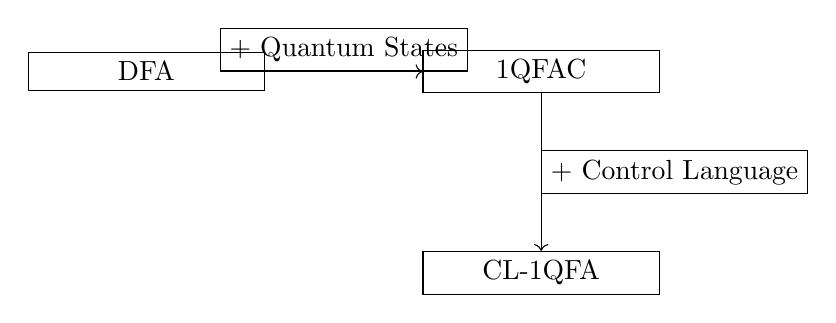
\begin{tikzpicture}[node distance=2cm, every node/.style={draw, rectangle, align=center, minimum width=3cm}]
    \node (DFA) {DFA};
    \node (1QFAC) [right=of DFA] {1QFAC};
    \node (CL1QFA) [below=of 1QFAC] {CL-1QFA};
    \draw[->] (DFA) -- (1QFAC) node[midway, above] {+ Quantum States};
    \draw[->] (1QFAC) -- (CL1QFA) node[midway, right] {+ Control Language};
\end{tikzpicture}
\caption{Evolution from classical DFA to hybrid QFAs. 1QFAC adds quantum states; CL-1QFA adds control languages.}
\label{fig:hybrid-evolution}
\end{figure}

%%%%%%%%%%%%%%%%%%%%%%%%%%%%%%%%%%%%%%%%%%%%%%%%%%%%%%%%%%%%%%
\section{Enhanced Models: Beyond Unitarity}
\label{sec:enhanced-comparison}
\begin{itemize}
    \item \textbf{\gls{eqfa}}:
    \begin{itemize}
        \item \textbf{Strengths}: Recognises non-regular languages (e.g., \( \{a^n b^n c^n\} \)) under unbounded error \cite{paschen2000quantum}.
        \item \textbf{Weaknesses}: Undecidable equivalence; requires ancilla qubits.
        \item \textbf{vs. PFA}: Subsumes PFA capabilities but with higher error rates.
    \end{itemize}
    
    \item \textbf{\gls{otqfa}}:
    \begin{itemize}
        \item \textbf{Strengths}: Models decoherence, recognizing regular languages with noise resilience.
        \item \textbf{Weaknesses}: Limited to isolated cut-point languages.
        \item \textbf{vs. 2PFA}: Similar expressive power but with quantum state efficiency.
    \end{itemize}
    
    \item \textbf{\gls{a-qfa}}:
    \begin{itemize}
        \item \textbf{Strengths}: Exponentially fewer states than \gls{nfa} for context-free languages like \( \{a^n b^n\} \).
        \item \textbf{Weaknesses}: Ancilla management complicates implementation.
        \item \textbf{vs. PDA}: Quantum parallelism replaces stack mechanics for specific languages.
    \end{itemize}
\end{itemize}

\begin{table}[ht]
\centering
\begin{tabular}{|l|c|c|c|}
\hline
\textbf{Model} & \textbf{Non-Regular Languages} & \textbf{Decoherence Handling} & \textbf{Ancilla Overhead} \\
\hline
EQFA & Yes (unbounded error) & Poor & High \\
OTQFA & No & Excellent & None \\
A-QFA & Yes (bounded error) & Moderate & Moderate \\
Classical 2PFA & Yes (e.g., \( L_{\text{eq}} \)) & N/A & N/A \\
\hline
\end{tabular}
\caption{Enhanced QFAs vs. classical probabilistic automata. EQFA trades ancilla overhead for non-regularity.}
\label{tab:enhanced-vs-classical}
\end{table}

%%%%%%%%%%%%%%%%%%%%%%%%%%%%%%%%%%%%%%%%%%%%%%%%%%%%%%%%%%%%%%
\section{Two-Way and Multi-Tape QFAs}
\label{sec:two-way-comparison}

\begin{itemize}
    \item \textbf{\gls{2qfa}}:
    \begin{itemize}
        \item \textbf{Strengths}: Recognises \( L_{\text{eq}} \) in linear time with bounded error \cite{yakaryilmaz2010succinctness}.
        \item \textbf{Weaknesses}: Quantum register scales with input length.
        \item \textbf{vs. 2DFA}: Exponential state advantage but impractical for large inputs.
    \end{itemize}
    
    \item \textbf{\gls{2qcfa}}:
    \begin{itemize}
        \item \textbf{Strengths}: Constant quantum states for \( L_{\text{pal}} \) \cite{ambainis2002quantum}.
        \item \textbf{Weaknesses}: Classical-quantum synchronization overhead.
        \item \textbf{vs. 2NFA}: Quantum interference replaces nondeterministic branching.
    \end{itemize}
    
    \item \textbf{\gls{ktqcfa}}:
    \begin{itemize}
        \item \textbf{Strengths}: Recognises \( k \)-tape dependencies (e.g., \( \{a^n b^n c^n\} \)) with \( O(1) \) quantum states \cite{zheng2012two}.
        \item \textbf{Weaknesses}: Head synchronization complexity \( \propto k \).
        \item \textbf{vs. Multi-Tape DFA}: Quantum parallelism reduces state complexity exponentially.
    \end{itemize}
\end{itemize}

\begin{figure}[ht]
\centering
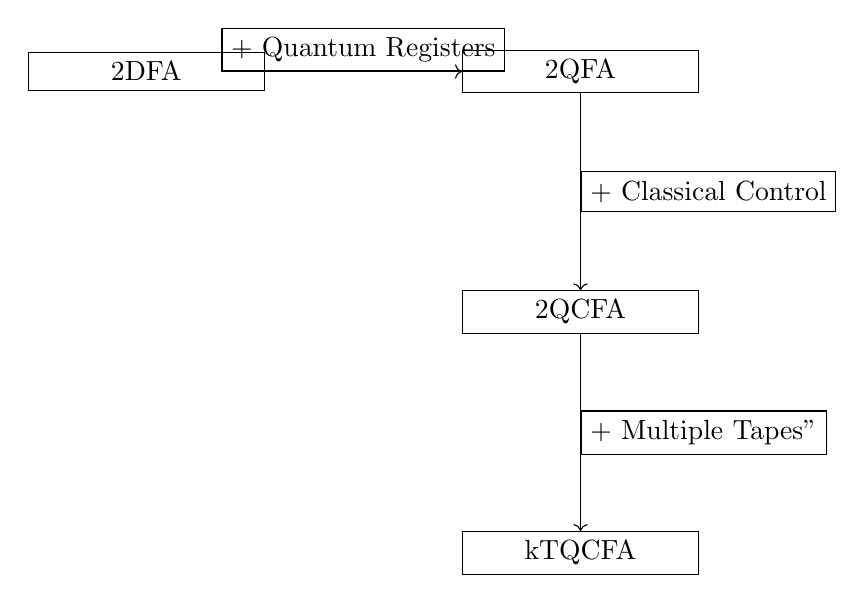
\begin{tikzpicture}[node distance=2.5cm, every node/.style={draw, rectangle, align=center, minimum width=3cm}]
    \node (2DFA) {2DFA};
    \node (2QFA) [right=of 2DFA] {2QFA};
    \node (2QCFA) [below=of 2QFA] {2QCFA};
    \node (kTQCFA) [below=of 2QCFA] {kTQCFA};
    \draw[->] (2DFA) -- (2QFA) node[midway, above] {+ Quantum Registers};
    \draw[->] (2QFA) -- (2QCFA) node[midway, right] {+ Classical Control};
    \draw[->] (2QCFA) -- (kTQCFA) node[midway, right] {+ Multiple Tapes"};
\end{tikzpicture}
\caption{Progression from classical two-way to quantum multi-tape models. Arrows indicate added features.}
\label{fig:two-way-progression}
\end{figure}

%%%%%%%%%%%%%%%%%%%%%%%%%%%%%%%%%%%%%%%%%%%%%%%%%%%%%%%%%%%%%%
\section{Interactive Models: Beyond Standard Computation}
\label{sec:interactive-comparison}

\begin{itemize}
    \item \textbf{\gls{qip}}:
    \begin{itemize}
        \item \textbf{Strengths}: Solves PSPACE-complete problems with quantum verifier-prover interaction \cite{zheng2015power}.
        \item \textbf{Weaknesses}: Requires fault-tolerant quantum channels.
        \item \textbf{vs. IP}: Exponential speedup for specific problems (e.g., group non-membership).
    \end{itemize}
    
    \item \textbf{\gls{qmip}}:
    \begin{itemize}
        \item \textbf{Strengths}: Recognises undecidable languages (e.g., \( \text{MIP}^* = \text{RE} \)) via multi-prover entanglement \cite{yamakami2014constant}.
        \item \textbf{Weaknesses}: Experimentally infeasible due to decoherence.
        \item \textbf{vs. MIP}: Unconditional security via quantum entanglement.
    \end{itemize}
\end{itemize}

\begin{table}[ht]
\centering
\begin{tabular}{|l|c|c|c|}
\hline
\textbf{Model} & \textbf{Complexity Class} & \textbf{Prover Type} & \textbf{Practicality} \\
\hline
QIP & PSPACE & Single (Quantum) & Moderate (needs error correction) \\
QMIP & RE & Multiple (Entangled) & Low (decoherence-sensitive) \\
Classical IP & PSPACE & Single (Classical) & High \\
\hline
\end{tabular}
\caption{Interactive QFAs vs. classical interactive proofs. QMIP’s expressiveness comes at experimental cost.}
\label{tab:interactive-vs-classical}
\end{table}

%%%%%%%%%%%%%%%%%%%%%%%%%%%%%%%%%%%%%%%%%%%%%%%%%%%%%%%%%%%%%%
\section{Overall Hierarchy and Recommendations}
\label{sec:hierarchy-summary}

\begin{figure}[ht]
\centering
\resizebox{\textwidth}{!}{%
\begin{tikzpicture}[node distance=1.5cm, every node/.style={draw, rectangle, align=center, minimum width=2.5cm, font=\footnotesize}]
    % One-way
    \node (MO1) {MO-1QFA};
    \node (MM1) [right=of MO1] {MM-1QFA};
    \node (LQFA) [right=of MM1] {LQFA};
    
    % Hybrid
    \node (1QFAC) [below=of MO1] {1QFAC};
    \node (CL1) [below=of MM1] {CL-1QFA};
    
    % Enhanced
    \node (EQFA) [below=of LQFA] {EQFA};
    \node (OTQFA) [right=of EQFA] {OTQFA};
    \node (AQFA) [right=of OTQFA] {A-QFA};
    
    % Two-way
    \node (2QFA) [above=of MO1] {2QFA};
    \node (2QCFA) [above=of MM1] {2QCFA};
    \node (kTQCFA) [above=of LQFA] {kTQCFA};
    
    % Interactive
    \node (QIP) [below=of EQFA, xshift=-2cm] {QIP};
    \node (QMIP) [right=of QIP] {QMIP};
    
    % Arrows
    \draw[->] (MO1) -- (MM1);
    \draw[->] (MM1) -- (LQFA);
    \draw[->] (MO1) -- (1QFAC);
    \draw[->] (MM1) -- (CL1);
    \draw[->] (LQFA) -- (EQFA);
    \draw[->] (1QFAC) -- (EQFA);
    \draw[->] (CL1) -- (OTQFA);
    \draw[->] (EQFA) -- (AQFA);
    \draw[->] (2QFA) -- (2QCFA);
    \draw[->] (2QCFA) -- (kTQCFA);
    \draw[->] (AQFA) -- (QIP);
    \draw[->] (QIP) -- (QMIP);
\end{tikzpicture}%
}
\caption{Comprehensive hierarchy of QFA models. Vertical arrows indicate increased expressiveness; horizontal arrows denote specialization. Interactive models (bottom) form a separate branch.}
\label{fig:full-hierarchy}
\end{figure}

\subsection*{Best and Worst Models by Feature}
\begin{itemize}
    \item \textbf{State Efficiency}: 
    \begin{itemize}
        \item \textbf{Best}: 1QFAC (constant quantum states for regular languages).  
        \item \textbf{Worst}: 2QFA (linear scaling quantum registers).
    \end{itemize}
    
    \item \textbf{Expressiveness}: 
    \begin{itemize}
        \item \textbf{Best}: QMIP (recognises recursively enumerable languages).  
        \item \textbf{Worst}: MO-1QFA (limited to reversible regular languages).
    \end{itemize}
    
    \item \textbf{Practicality}: 
    \begin{itemize}
        \item \textbf{Best}: MM-1QFA (bounded error, simple implementation).  
        \item \textbf{Worst}: kTQCFA (high synchronization overhead).
    \end{itemize}
\end{itemize}

%%%%%%%%%%%%%%%%%%%%%%%%%%%%%%%%%%%%%%%%%%%%%%%%%%%%%%%%%%%%%%
\section*{Conclusion}
The QFA landscape reveals a trade-off between expressiveness and practicality. While models like QMIP and 2QFA push quantum advantages to theoretical limits, hybrid models like 1QFAC and 2QCFA offer near-term viability. Future work should prioritise error correction for enhanced models and experimental validation of interactive protocols.
\chapter{Conclusion}
\label{chap:conclusion}

This thesis systematically analyzed \glsentrylongpl{qfa} by comparing them to classical models. The goal was to clarify where quantum advantages exist, quantify their costs, and identify practical limitations.

Three key results emerged. First, \glsentrylongpl{1qfa} such as \gls{mm-1qfa} achieve exponential state reduction over classical automata for regular languages but require careful error management. Second, Two-way and Hybrid models like \gls{2qcfa} extend recognition to non-regular languages (e.g., $\{a^n b^n\}$) with constant quantum memory, though classical control introduces synchronization overhead. Third, generalized models and interactive protocols reveal fundamental trade-offs: while they theoretically recognize complex languages, their reliance on noise modeling or multi-prover coordination makes them experimentally challenging.

These findings have concrete implications. For algorithm designers, hybrid models like \glspl{1qfac} offer a pragmatic balance—using minimal quantum resources while retaining classical reliability. For hardware developers, the analysis underscores the need for error correction tailored to automata (e.g., handling decoherence in \glspl{mo-1qfa}'s unitary evolution). The undecidability of equivalence problems for many \glspl{qfa} also highlights a theoretical barrier: verifying quantum automata behavior may require new formal methods.

Future work should prioritize practical over theoretical novelty. Compiling \glspl{qfa} into quantum circuits would test their real-world viability, while equivalence studies between \glspl{qfa} and \glspl{qtm} could unify computational models. For industry, implementing \glspl{2qcfa} on \gls{nisq} devices to solve simple context-sensitive problems (e.g., \glsentryshort{xml} validation) might demonstrate near-term utility.

In summary, this work clarifies what quantum automata can and cannot do today. It provides a roadmap for leveraging their strengths—state efficiency and parallelism—while cautioning against underestimating their fragility. The path forward lies in bridging formal theory with engineering constraints, not chasing abstract generality.


\printglossary[title={Abbreviations},type=acronym,style=long]
\appendix
\printbibliography

\printindex

\chapter*{Acknowledgments}

Above all, this journey has been immensely rewarding, even though it was demanding and at times exhausting.

Since I began my studies at the University of Camerino, Michele Loreti has remained a steady mentor, and I am deeply grateful for his guidance.

I also value Marcello Bonsangue's generosity, openness, constant good humour, and sharp feedback.

Thank you to the LIACS staff and PhD students for creating a friendly and engaging environment. You made every day interesting and enjoyable, from lively whiteboard sessions to endless coffee breaks.

To my family: thank you for your steady support and for always being there. Mum, you have been my unfailing reference in all matters, ready with practical advice and help whenever I needed it.

To my friends in Camerino: thank you for turning that small town into the centre of the universe. A special shout-out to Alice, my anchor during the toughest moments.

Valentijn, thank you for making my time in the Netherlands even lovelier and for giving me a sense of home there. You stood by me during those life-changing months, bringing peace and calm when I needed them most.

I'm grateful to everyone I've met. Whether you encouraged me or pushed me, you influenced who I am today.

Lastly, I want to thank the version of me who set out on this adventure three years ago. Even without a clear destination, you kept your energy, curiosity, and resolve. I'm proud of who you've become; it was hard, but it was worth it.

\end{document}